% Created by tikzDevice version 0.12.3.1 on 2021-12-02 12:52:40
% !TEX encoding = UTF-8 Unicode
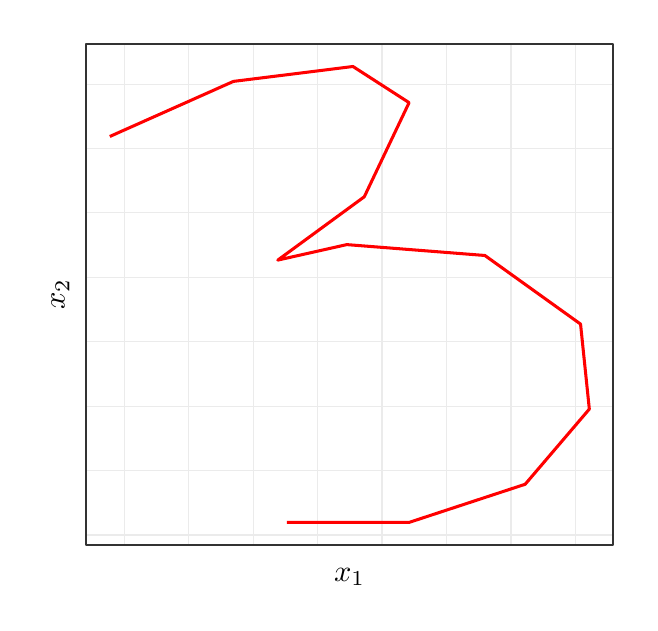
\begin{tikzpicture}[x=1pt,y=1pt]
\definecolor{fillColor}{RGB}{255,255,255}
\begin{scope}
\definecolor{drawColor}{RGB}{255,255,255}
\definecolor{fillColor}{RGB}{255,255,255}

\path[draw=drawColor,line width= 0.6pt,line join=round,line cap=round,fill=fillColor] (  0.00,  4.72) rectangle (216.81,212.09);
\end{scope}
\begin{scope}
\definecolor{fillColor}{RGB}{255,255,255}

\path[fill=fillColor] ( 20.71, 25.43) rectangle (211.31,206.59);
\definecolor{drawColor}{gray}{0.92}

\path[draw=drawColor,line width= 0.3pt,line join=round] ( 20.71, 52.25) --
	(211.31, 52.25);

\path[draw=drawColor,line width= 0.3pt,line join=round] ( 20.71, 98.85) --
	(211.31, 98.85);

\path[draw=drawColor,line width= 0.3pt,line join=round] ( 20.71,145.46) --
	(211.31,145.46);

\path[draw=drawColor,line width= 0.3pt,line join=round] ( 20.71,192.06) --
	(211.31,192.06);

\path[draw=drawColor,line width= 0.3pt,line join=round] ( 57.95, 25.43) --
	( 57.95,206.59);

\path[draw=drawColor,line width= 0.3pt,line join=round] (104.55, 25.43) --
	(104.55,206.59);

\path[draw=drawColor,line width= 0.3pt,line join=round] (151.15, 25.43) --
	(151.15,206.59);

\path[draw=drawColor,line width= 0.3pt,line join=round] (197.76, 25.43) --
	(197.76,206.59);

\path[draw=drawColor,line width= 0.6pt,line join=round] ( 20.71, 28.95) --
	(211.31, 28.95);

\path[draw=drawColor,line width= 0.6pt,line join=round] ( 20.71, 75.55) --
	(211.31, 75.55);

\path[draw=drawColor,line width= 0.6pt,line join=round] ( 20.71,122.16) --
	(211.31,122.16);

\path[draw=drawColor,line width= 0.6pt,line join=round] ( 20.71,168.76) --
	(211.31,168.76);

\path[draw=drawColor,line width= 0.6pt,line join=round] ( 34.65, 25.43) --
	( 34.65,206.59);

\path[draw=drawColor,line width= 0.6pt,line join=round] ( 81.25, 25.43) --
	( 81.25,206.59);

\path[draw=drawColor,line width= 0.6pt,line join=round] (127.85, 25.43) --
	(127.85,206.59);

\path[draw=drawColor,line width= 0.6pt,line join=round] (174.46, 25.43) --
	(174.46,206.59);
\definecolor{drawColor}{RGB}{255,0,0}

\path[draw=drawColor,line width= 1.1pt,line join=round] ( 93.33, 33.66) --
	(137.66, 33.66) --
	(179.47, 47.40) --
	(202.65, 74.56) --
	(199.48,105.28) --
	(164.91,130.07) --
	(115.02,134.00) --
	( 90.08,128.40) --
	(121.33,151.28) --
	(137.52,185.30) --
	(117.24,198.36) --
	( 74.04,192.97) --
	( 29.38,173.07);
\definecolor{drawColor}{gray}{0.20}

\path[draw=drawColor,line width= 0.6pt,line join=round,line cap=round] ( 20.71, 25.43) rectangle (211.31,206.59);
\end{scope}
\begin{scope}
\definecolor{drawColor}{RGB}{0,0,0}

\node[text=drawColor,anchor=base,inner sep=0pt, outer sep=0pt, scale=  1.10] at (116.01, 12.35) {$x_1$};
\end{scope}
\begin{scope}
\definecolor{drawColor}{RGB}{0,0,0}

\node[text=drawColor,rotate= 90.00,anchor=base,inner sep=0pt, outer sep=0pt, scale=  1.10] at ( 13.08,116.01) {$x_2$};
\end{scope}
\end{tikzpicture}
